%
% sweep.tex -- template for standalon tikz images
%
% (c) 2019 Prof Dr Andreas Müller, Hochschule Rapperswil
%
\documentclass[tikz]{standalone}
\usepackage{amsmath}
\usepackage{times}
\usepackage{txfonts}
\usepackage{pgfplots}
\usepackage{csvsimple}
\usetikzlibrary{arrows,intersections,math}
\begin{document}
\begin{tikzpicture}[>=latex]

\pgfmathparse{0.6*(9/16)*12}
\xdef\s{\pgfmathresult}

\node at (6,{6*9/16}) {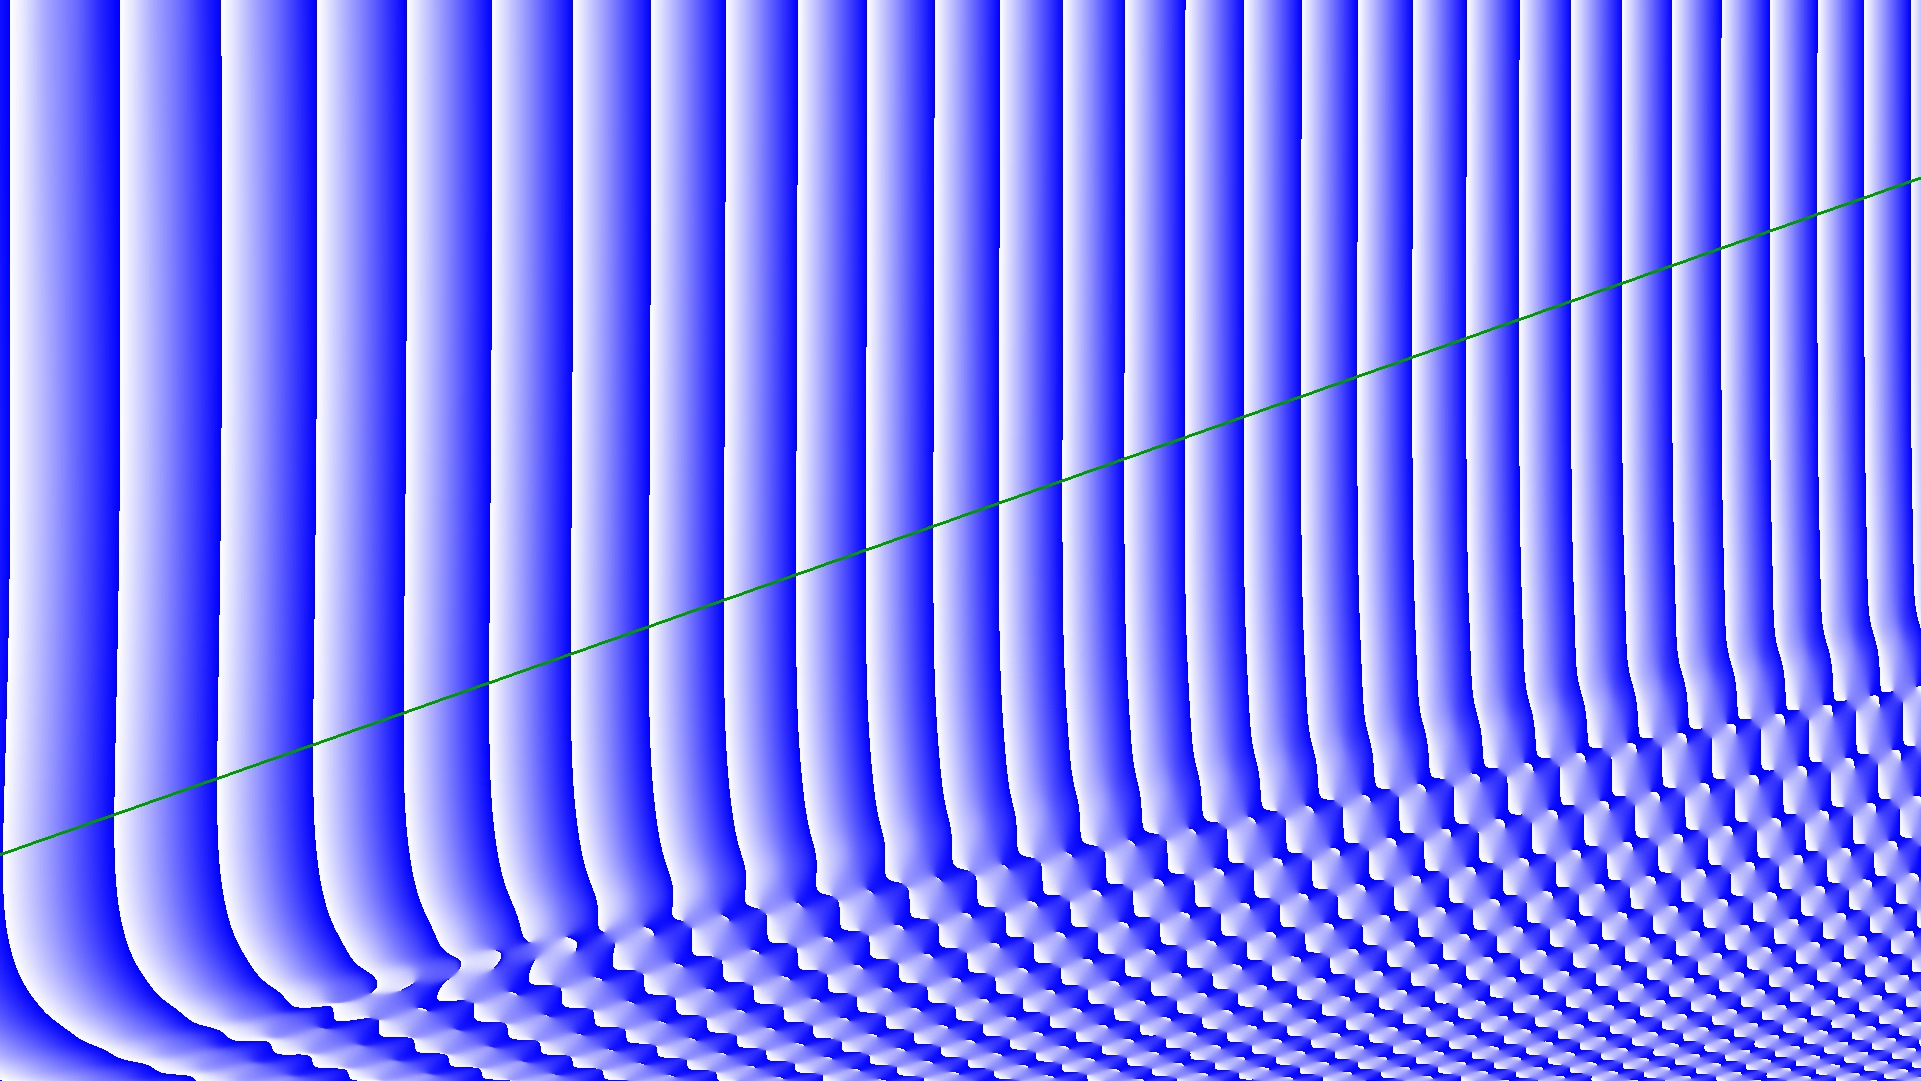
\includegraphics[width=12cm]{sweep-phase.jpg}};
\draw[->,line width=0.7pt] (-0.1,0)--(12.3,0) coordinate[label={$b$}];
\draw[->,line width=0.7pt] (0,-0.1)--(0,{12*9/16+0.3})
	coordinate[label={right:$1/a$}];
\foreach \x in {-12,...,13}{
	\draw[line width=0.7pt]
		({(\x+13)*(12/26)},-0.1)--({(\x+13)*(12/26)},0.1);
}
%        double  amin = 0.5;
%        double  amax = 3;
\draw[line width=0.7pt] (-0.1,0)--(0.1,0);
\node at (-0.1,0) [left] {$a=3$};
\draw[line width=0.7pt] (-0.1,{(1/2-1/3)*\s})--(0.1,{(1/2-1/3)*\s});
\node at (-0.1,{(1/2-1/3)*\s}) [left] {$a=2$};
\draw[line width=0.7pt] (-0.1,{(1-1/3)*\s})--(0.1,{(1-1/3)*\s});
\node at (-0.1,{(1-1/3)*\s}) [left] {$a=1$};
\draw[line width=0.7pt] (-0.1,{12*(9/16)})--(0.1,{12*(9/16)});
\node at (-0.1,{12*(9/16)}) [left] {$a=0.5$};

\begin{scope}[yshift=7.5cm]
\node at (6,{6*9/16}) {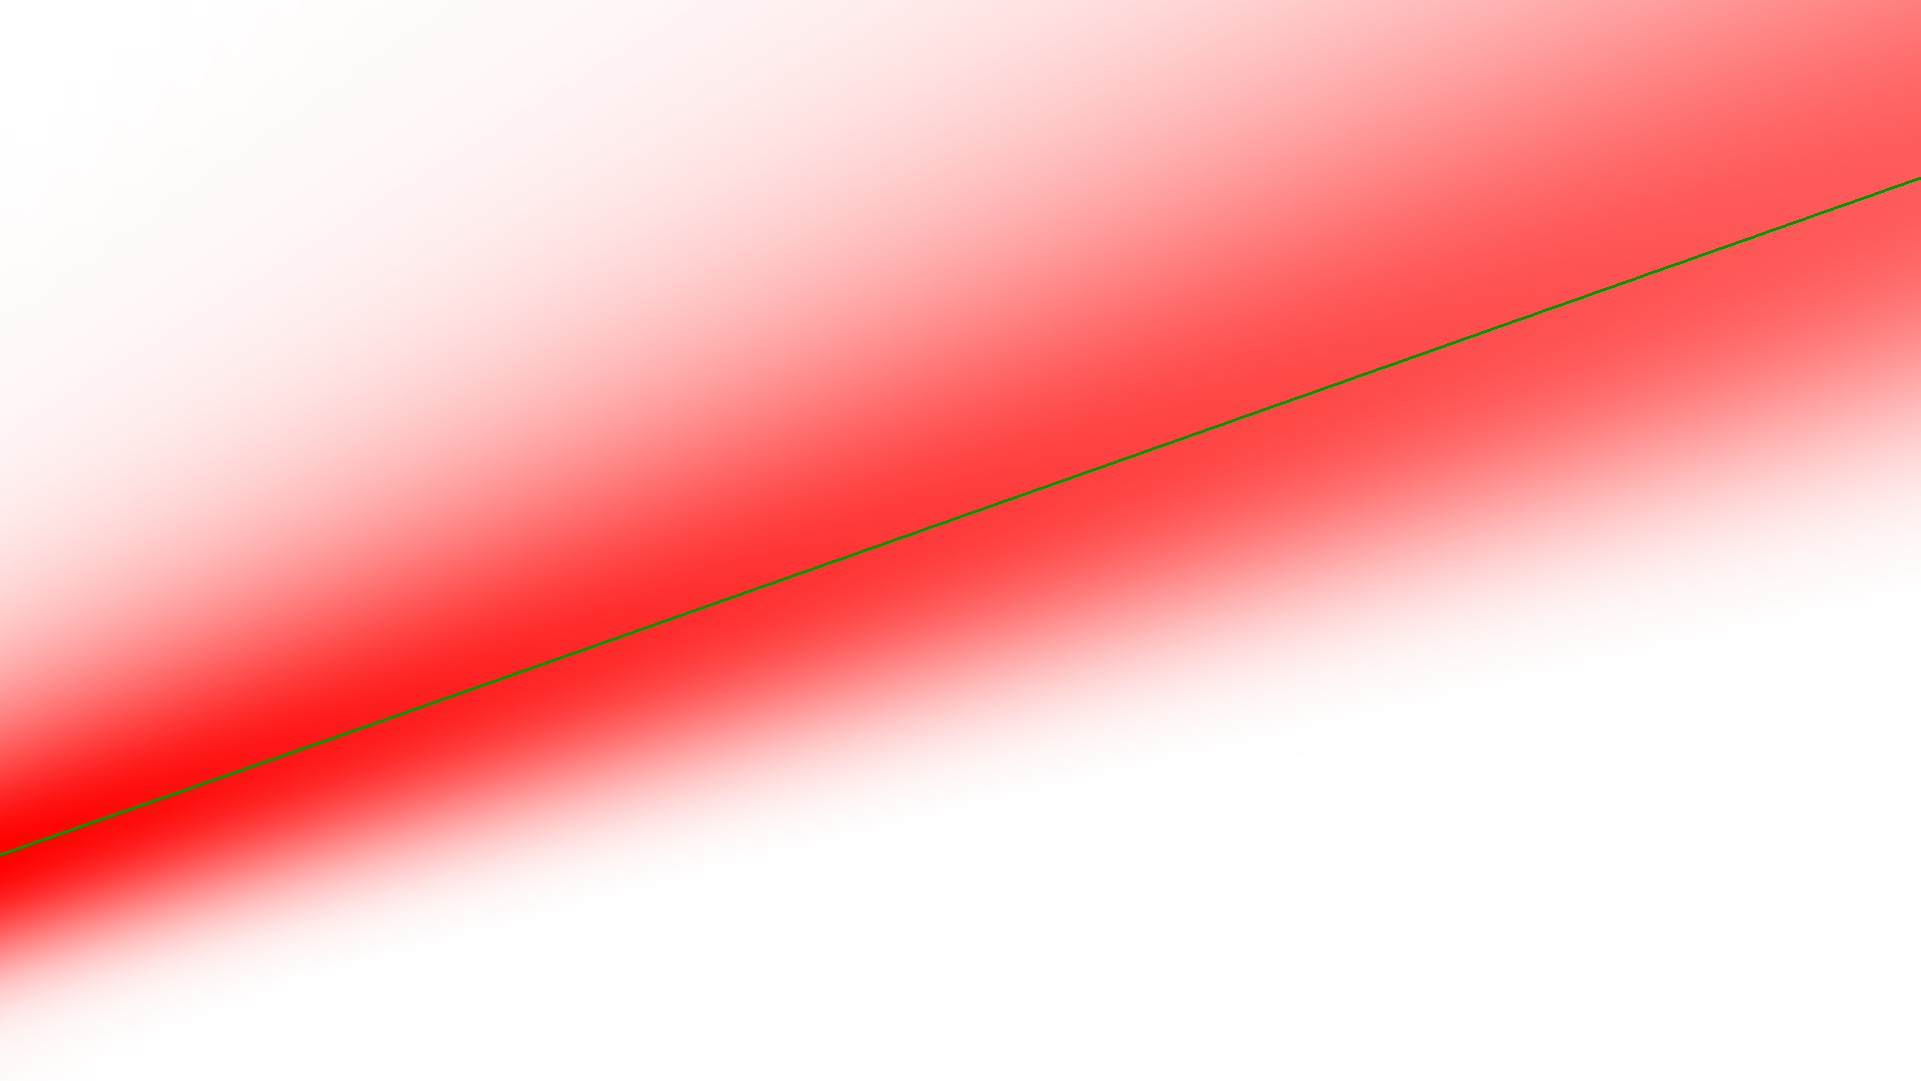
\includegraphics[width=12cm]{sweep-abs.jpg}};
\draw[->,line width=0.7pt] (-0.1,0)--(12.3,0) coordinate[label={$b$}];
\draw[->,line width=0.7pt] (0,-0.1)--(0,{12*9/16+0.3})
	coordinate[label={right:$1/a$}];
\foreach \x in {-12,...,13}{
	\draw[line width=0.7pt]
		({(\x+13)*(12/26)},-0.1)--({(\x+13)*(12/26)},0.1);
}
\draw[line width=0.7pt] (-0.1,0)--(0.1,0);
\node at (-0.1,0) [left] {$a=3$};
\draw[line width=0.7pt] (-0.1,{(1/2-1/3)*\s})--(0.1,{(1/2-1/3)*\s});
\node at (-0.1,{(1/2-1/3)*\s}) [left] {$a=2$};
\draw[line width=0.7pt] (-0.1,{(1-1/3)*\s})--(0.1,{(1-1/3)*\s});
\node at (-0.1,{(1-1/3)*\s}) [left] {$a=1$};
\draw[line width=0.7pt] (-0.1,{12*(9/16)})--(0.1,{12*(9/16)});
\node at (-0.1,{12*(9/16)}) [left] {$a=0.5$};
\end{scope}

\begin{scope}[yshift=-1.8cm]
\draw[color=red,line width=1pt]
	plot[domain=-13:13,samples=4000]
		({(\x+13)*(12/26)},{sin((\x+13)*(4+(0.2*(\x+13)))*(180/3.1415))});
\draw[->,line width=0.7pt] (-0.1,0)--(12.3,0) coordinate[label={$t$}];
\draw[->,line width=0.7pt] (0,-1.1)--(0,1.3) coordinate[label={right:$f(t)$}];
\foreach \x in {-12,...,13}{
	\draw[line width=0.7pt]
		({(\x+13)*(12/26)},-0.1)--({(\x+13)*(12/26)},0.1);
}
\end{scope}

\end{tikzpicture}
\end{document}

